\newpage
\section{Mateusz Zawieracz}
\label{sec:matzaw}

\par
The stocky, short-legged appearance of penguins has endeared them to people worldwide. They range from about 35 cm (14 inches) in height and approximately 1 kg (about 2 pounds) in weight in the blue, or fairy, penguin (Eudyptula minor) to 115 cm (45 inches) and 25 to 40 kg (55 to 90 pounds) in the emperor penguin (Aptenodytes forsteri). Most are black on the back and white below, often with lines of black across the upper breast or spots of white on the head. Colour is rare, being limited to red or yellow irises of the eye in some species; red beaks or feet in a few; yellow brow tufts in the three species of Eudyptes; and orange and yellow on the head, neck, and breast in the emperor and king (A. patagonica) penguins.

\par
The total populations of some species, such as the emperor, are estimated in the hundreds of thousands, but most species of smaller penguins certainly run into the millions. Immense island breeding colonies, some teeming with hundreds of thousands of nesting pairs, represent a large potential food resource, but the economic importance of penguins is negligible. Nineteenth-century whalers and seal hunters visited some colonies for meat and eggs, and a penguin oil industry once took large numbers of the birds. By the early 20th century, however, this exploitation was no longer profitable, and most colonies were left alone or actively protected. Some species are now increasing in numbers, apparently as a result of the mid-20th century’s decimation of Antarctic whales, which compete with penguins for the krill (minute crustaceans) on which both feed. Penguin populations, however, are highly vulnerable to changes in climate and ocean temperature, including recent global warming. Penguins also are very sensitive to depletion of local fish populations by humans.



Here is a picutre of a penguin (see Figure~\ref{fig:penguin}).

\begin{figure}[htbp] 
    \centering
    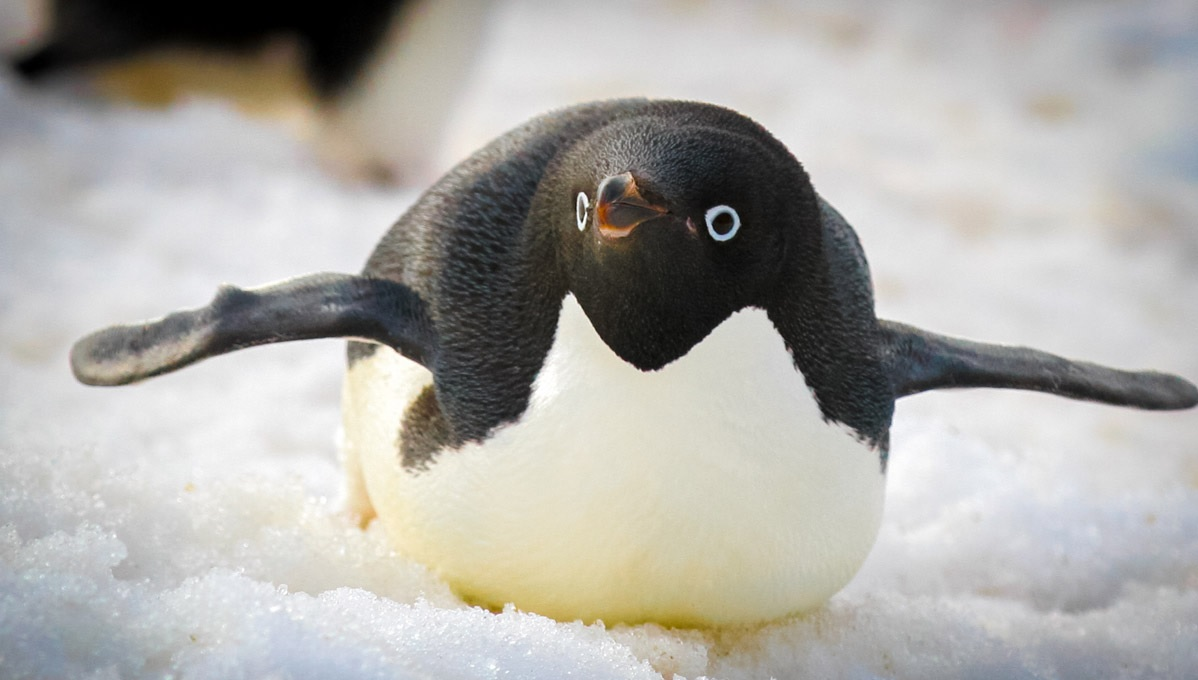
\includegraphics[width=0.6\textwidth]{pictures/penguin.jpg}
    \caption{The penguin is \textbf{gliding}.}
    \label{fig:penguin}
\end{figure}
\newpage
Table ~\ref{tab:penguins} represents penguin population in certain countries.
\begin{table}[htbp]
\centering
\renewcommand{\arraystretch}{1.2} % Adjust row height
\setlength{\tabcolsep}{12pt} % Adjust column spacing
\begin{tabular}{|c|r|}
\hline
\textbf{Country} & \textbf{Penguin Population} \\ \hline
Chile            & 13,000,000                  \\ \hline
Falkland Islands & 1,200,000                   \\ \hline
Argentina        & 1,000,000                   \\ \hline
Australia        & 500,000                     \\ \hline
New Zealand      & 500,000                     \\ \hline
South Africa     & 60,000                      \\ \hline
Namibia          & 26,000                      \\ \hline
Brazil           & 10,000                      \\ \hline
Peru             & 4,000                       \\ \hline
\end{tabular}
\caption{Penguin Populations by Country}
\label{tab:penguins}
\end{table}


This is an equation related to penguins:
\begin{equation}
    pegui = \sum_{n=0}^{\infty}(-1)^n \frac{4n}{2n+1}
\end{equation}

Penguins could also slide on $\frac{\arcsin{x}}{2}$ or $\frac{\arccos{x}}{4}$

Penguins are:
\begin{itemize}
    \item white
    \item black
    \item cute
\end{itemize}
Penguins are NOT:
\begin{enumerate}
    \item fat
    \item ugly
    \item scary
\end{enumerate}